\documentclass{beamer}

% Top-aligning columns within a top-aligned frame
% https://tex.stackexchange.com/questions/16447/beamer-top-aligning-columns-within-a-top-aligned-frame
\makeatletter
\newenvironment{myitemize}{%
   \setlength{\topsep}{0pt}
   \setlength{\partopsep}{0pt}
   \renewcommand*{\@listi}{\leftmargin\leftmargini \parsep\z@ \topsep\z@ \itemsep\z@}
   \let\@listI\@listi
   \itemize
}{\enditemize}
\makeatother  

\usepackage[USenglish]{babel}
\usepackage[utf8]{inputenc}
\usepackage{amssymb, amsmath}
\usepackage{bm}
\usepackage{color}
\usepackage{tikz}
\usepackage{url}

\definecolor{links}{HTML}{2A1B81}
\hypersetup{colorlinks,linkcolor=,urlcolor=links}

\usetheme{Boadilla}

\bibliographystyle{apalike}
% make bibliography entries smaller
%\renewcommand\bibfont{\scriptsize}
% Now get rid of all the colours
\setbeamercolor*{bibliography entry title}{fg=black}
\setbeamercolor*{bibliography entry author}{fg=black}
\setbeamercolor*{bibliography entry location}{fg=black}
\setbeamercolor*{bibliography entry note}{fg=black}

\newcommand{\lnorm}[1]{\left\lVert#1\right\rVert^2}
\newcommand{\norm}[1]{\left\lVert#1\right\rVert}

% and kill the abominable icon
\setbeamertemplate{bibliography item}{}

\begin{document}
\title[Anomaly Detection (AD)]{Rethinking Assumptions in Deep Anomaly Detection}  
\author{Radek Bartyzal}
\date{16. 6. 2020} 
\institute{GLAMI AI}

\frame{\titlepage} 

%--------- END Frame 12 -------------
\begin{frame}{Anomaly Detection (AD)}

\textbf{Unsupervised}
\begin{itemize}
\item classic approach
\item we usually have unlabeled corpus of mostly nominal data
\end{itemize}


\textbf{Semi-supervised}
\begin{itemize}
\item = AD with negative examples
\item = like unsupervised but push negative samples away from positive
\item OE = outlier exposure = enrich dataset with data known to be anomalous = download random images
\end{itemize}

\textbf{Supervised}
\begin{itemize}
\item usually small number of known anomaly samples
\item tricky to construct dataset that covers "everything else" as anomaly
\end{itemize}


\end{frame}

%--------- END Frame 12 -------------
\begin{frame}{Decision boundaries}

\begin{figure}[h]
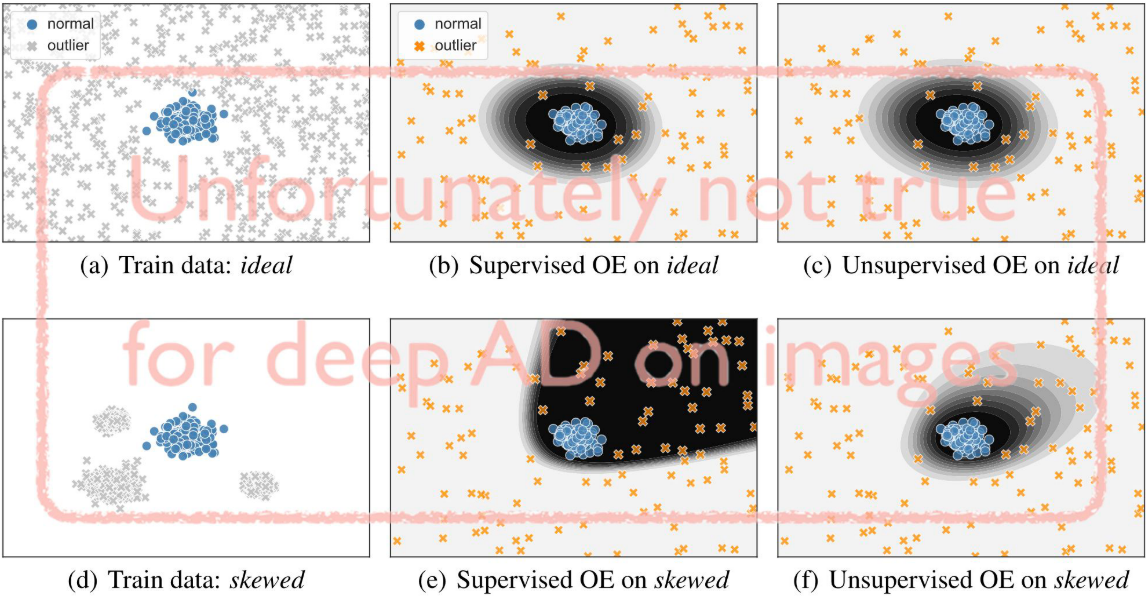
\includegraphics[width=\textwidth]{img/boundary}
\caption{Supervised methods look for a clean decision boundary. Unsupervised / semi-sup. = clustering.}
\end{figure}

\end{frame}

%--------- END Frame 12 -------------
\begin{frame}{Overview of methods}
\begin{itemize}
\item autoencoders trained on nominal data, where samples not reconstructed well are deemed anomalous

\item use of OE: train net to predict uniform distribution (=random) for all outliers (=random images/data) = we expect that the nominal data are not random while everything else is

\item \textbf{Unsupervised} deep version of support vector data description (Deep SVDD) Network is trained to map nominal samples to a center c: 
\begin{figure}[h]
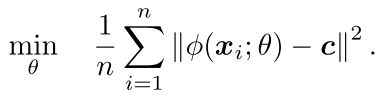
\includegraphics[width=0.4\textwidth]{img/svdd}
\end{figure}

\item Deep \textbf{Semi-supervised} Anomaly Detection (Deep SAD). Deep SAD trains a network to concentrate nominal data near a predetermined center and maps anomalous samples away from that center.

\end{itemize}
\end{frame}
%--------- END Frame 12 -------------
\begin{frame}{Proposed method}

Change Deep SAD to \textbf{Hypersphere classifier (HSC)} = cross-entropy classification that concentrates nominal samples together and pushes anomalies away = still unsupervised.

\vfill

Cross entropy:

\begin{figure}[h]
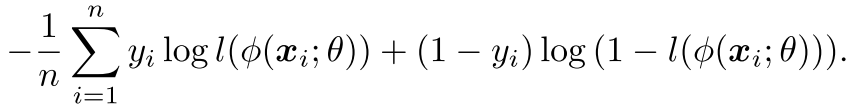
\includegraphics[width=0.8\textwidth]{img/eq1}
\end{figure}

Use $l(z) = \exp (- \Vert z \Vert ^2)$:
\begin{figure}[h]
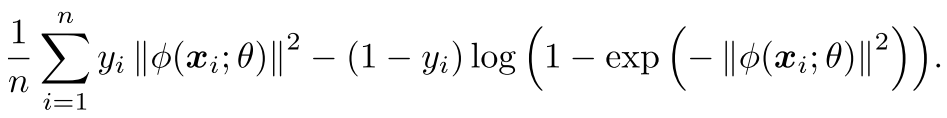
\includegraphics[width=0.8\textwidth]{img/eq2}
\end{figure}
\end{frame}
%--------- END Frame 12 -------------
\begin{frame}{Proposed method}
\begin{figure}[h]
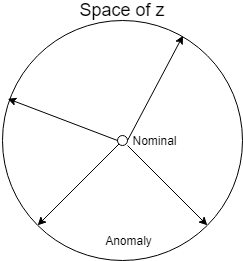
\includegraphics[width=0.4\textwidth]{img/radial_loss}
\caption{$z$ is the output of the ANN.}
\end{figure}

Anomaly score $s(x) = \Vert ANN(x) \Vert ^2$.

\end{frame}
%--------- END Frame 12 -------------
\begin{frame}{Goals}
This paper challenges following common assumptions:
\begin{itemize}
\item Many (thousands) samples are needed for a deep method to understand a class of data.
\item Anomalies are unconcentrated and thus inherently difficult to characterize with data.
\item Therefore unsupervised approach is better than supervised.
\end{itemize}

\end{frame}

%--------- END Frame 12 -------------

\begin{frame}{Experiments}

\textbf{One vs. Rest Benchmark} = “one” class (e.g, digit 0) as being nominal and the “rest” classes (e.g., digits 1–9) as being anomalous at test time.

\vfill

\textbf{Datasets:}
\begin{itemize}
\item MNIST - with EMNIST-Letters as OE data
\item CIFAR10 - with Tiny Images (80MTI) without CIFAR as OE
\item ImageNet 1K - with ImageNet-22K without 1K as OE
\end{itemize}

\vfill

\textbf{Models:}
\begin{itemize}
\item Unsupervised: SVDD, state-of-the-art methods = GEO, IT
\item Semi-Supervised: HSC
\item Supervised: standard binary cross-entropy classifier: BCE
\end{itemize}


\end{frame}

%--------- END Frame 12 -------------
\begin{frame}{Experiments: CIFAR10 one vs rest}
\begin{figure}[h]
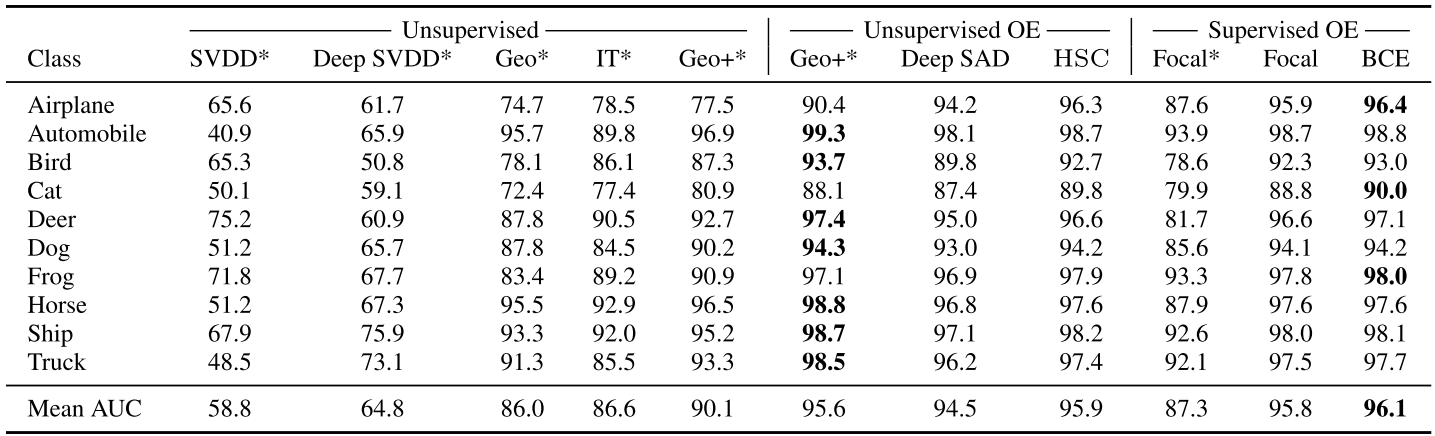
\includegraphics[width=\textwidth]{img/table1}
\caption{BCE performs better than SOTA unsupervised OE.}
\end{figure}

\end{frame}
%--------- END Frame 12 -------------
\begin{frame}{Experiments: CIFAR10 one vs rest}
\begin{figure}[h]
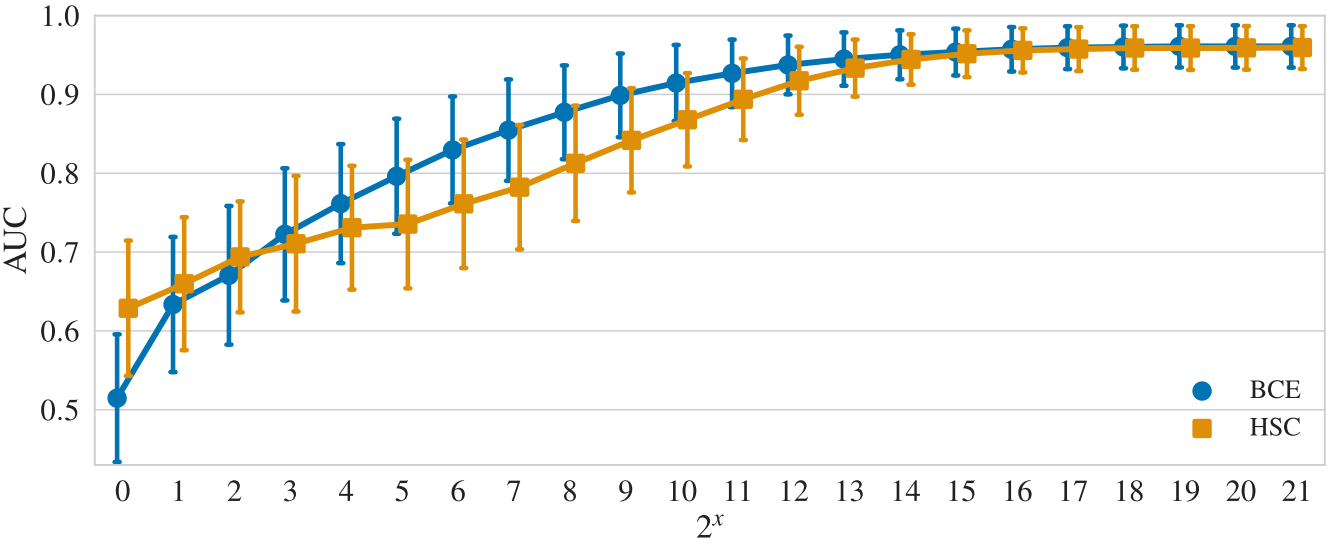
\includegraphics[width=\textwidth]{img/bce_vs_hsc}
\caption{Detection performance in mean AUC in \% (over 10 classes with 10 seeds per class) on the CIFAR-10 one vs. rest benchmark when varying the number of 80MTI OE samples. 32 OE samples is enough.}
\end{figure}
\end{frame}
%--------- END Frame 12 -------------
\begin{frame}{Experiments: ImageNet one vs rest}
\begin{figure}[h]
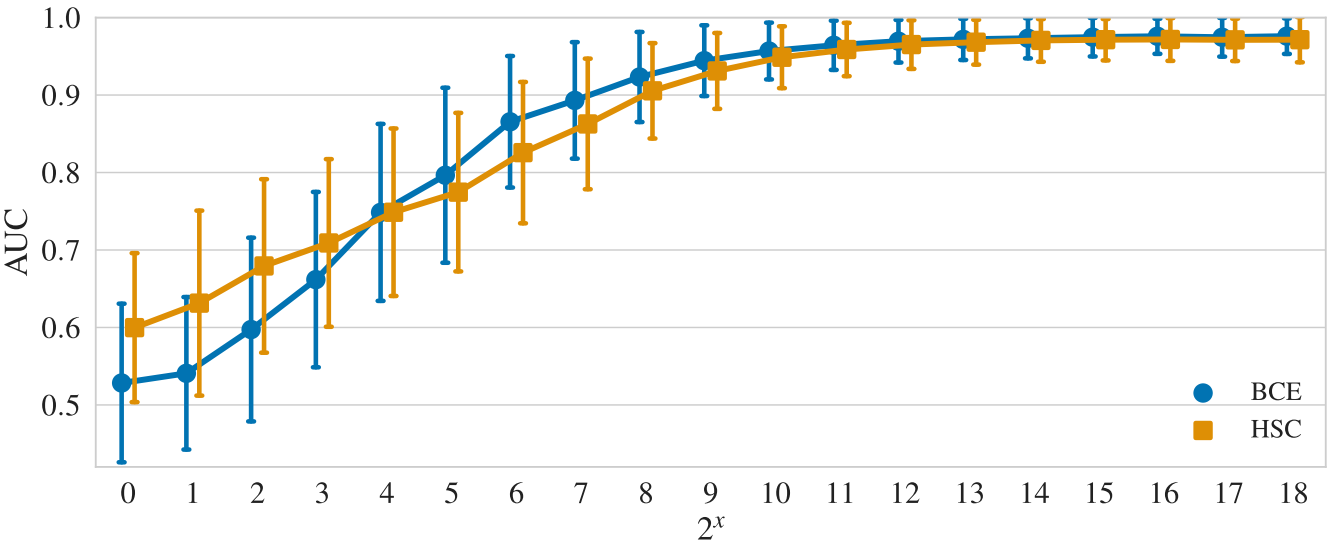
\includegraphics[width=\textwidth]{img/bce_vs_hsc_imagenet}
\caption{Detection performance in mean AUC in \% (over 30 classes with 5 seeds per class) on the ImageNet-1K one vs. rest benchmark when varying the number of ImageNet-22K OE samples. 64 OE samples is enough.}
\end{figure}
\end{frame}
%--------- END Frame 12 -------------
\begin{frame}{Experiments: ImageNet blurring}
\begin{figure}[h]
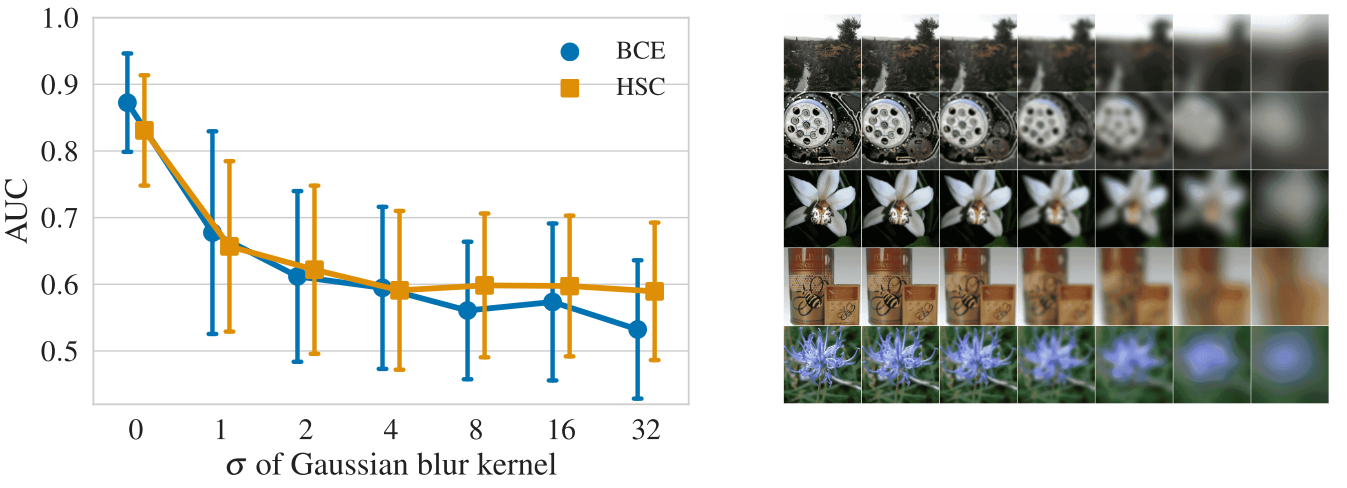
\includegraphics[width=\textwidth]{img/gauss}
\caption{Detection performance in mean AUC on ImageNet when the OE data samples become increasingly blurred with a Gaussian kernel for having $2^6$ = 64 OE samples (left). An example of the various degrees of blurring is shown on the right. The abrupt decrease in AUC suggests the exceptional informativeness of OE on images is due to the multiscale structure of images.}
\end{figure}
\end{frame}
%--------- END Frame 12 -------------
\begin{frame}{Results}

Key difference between classic AD and deep image AD is the presence of information at multiple spatial scales in images
= small number of images contains a lot of information.

\vfill

\textbf{Supporting evidence:}
\begin{itemize}
\item advantage of supervised OE over unsupervised OE is most evident on ImageNet, a high-resolution dataset. Smaller on CIFAR10 and nonexistent at MNIST.
\item blurring ImageNet images = corrupting small scale features = drastic reduction in performance  
\end{itemize}

\vfill

\textbf{Other results:}
\begin{itemize}
\item very large amount of OE examples = unsupervised OE and supervised OE are equal
\end{itemize}

\end{frame}
%--------- END Frame 12 -------------
\begin{frame}{Sources}
\begin{thebibliography}{0}

  \bibitem[1]{cit:paper} 1. Ruff, Lukas, et al. "Rethinking Assumptions in Deep Anomaly Detection." arXiv preprint arXiv:2006.00339 (2020). \url{https://arxiv.org/abs/2006.00339} 
  
\end{thebibliography}

\end{frame}

 
\end{document}
